The TRITIUM-IFIC-0 prototype was the first prototype developed in the TRITIUM experiment to check the feasibility of the technology proposed by TRITIUM, that is, to verify that is using plastic scintillating fibers to detect tritium in water with good sensitivity.

As liquid radioactive sources were involved, a special attention was paid to radiation safety in the design of the first prototype.

TRITIUM-IFIC-0 consists of a bundle of 35 fibers, shown in Figure \ref{fig:FiberBundleOfTritiumIFIC0}, of $20~\cm$ length, which were cleaved and polished with the techniques reported in section \ref{subsec:SurfaceConditioningProcess}. This bundle has metalic pieces located in both ends, shown in Figure \ref{subfig:MetalicPieceFiberBunchTritiumIFIC0} for attaching it to the prototype vessel. The fiber bundle was placed inside of a vessel, made of PVC\footnote{Polyvinyl Chloride, PVC}  since it is a safe widely used material. This vessel, shown in Figure \ref{fig:TritiumIFIC0}, was designed in a U-shape to improve the radiological safety, although this shape was not the most appropriate for tritium detection, as we learned afterwards. As can be seen in Figure \ref{fig:TritiumIFIC0}, a frame of methacrylate and steel was designed and built to hold the prototype. Two calibrated Hamamatsu R8520-460 PMTs \cite{DataSheetPMTs} were optically coupled to the fiber bundle ends using optical grease \cite{OpticalGrease}. The voltage divider circuit of these PMTs is shown in Figure  \ref{fig:VoltageDividerCircuit}. The high voltage was set to $-800~\volt$, at which the gain are $1.26 \cdot{} 10^6$ and $1.01 \cdot{} 10^6$, and the quantum efficiency $29.76\%$ and $28.66\%$, respectively. The two PMTs were read out in coincidence mode, using the electronics circuit shown in Figure \ref{subfig:ElectronicConfiguraiton2PMT}.

\begin{figure}
\centering
    \begin{subfigure}[b]{0.5\textwidth}
    \centering
    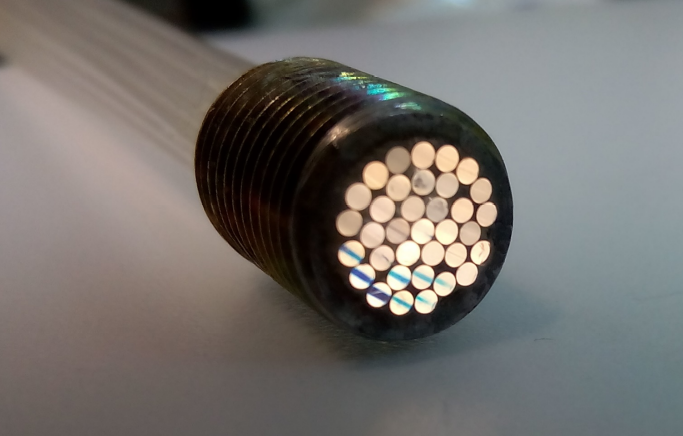
\includegraphics[width=\textwidth]{5Prototypes/52PreliminarPrototypes/521TritiumIFIC0/Metalic_piece_of_fiber_bundle.png}  
    \caption{\label{subfig:MetalicPieceFiberBunchTritiumIFIC0}}
    \end{subfigure}
    \hfill
    \begin{subfigure}[b]{0.4\textwidth}
    \centering
    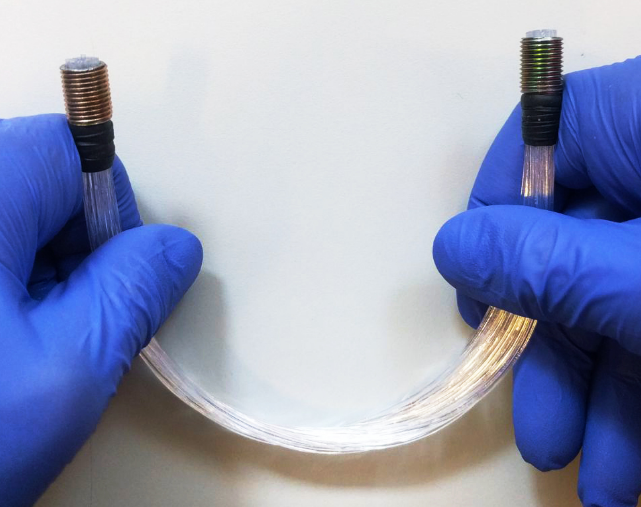
\includegraphics[width=\textwidth]{5Prototypes/52PreliminarPrototypes/521TritiumIFIC0/FiberBundleBent.png}  
    \caption{\label{subfig:FiberBunchTritiumIFIC0Bent}}
    \end{subfigure}
    \hfill
    \begin{subfigure}[b]{0.7\textwidth}
    \centering
    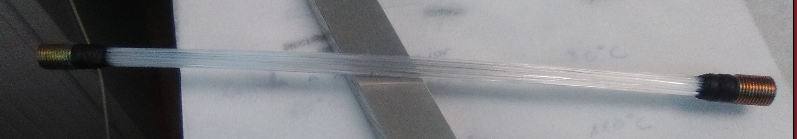
\includegraphics[width=\textwidth]{5Prototypes/52PreliminarPrototypes/521TritiumIFIC0/FiberBundleStraight.png}  
    \caption{\label{subfig:FiberBunchTritiumIFIC0}}
    \end{subfigure}
 \caption{a) Metallic piece of the fiber bundle. b) and c) Bundle of $35$ fibers, the length of which is $20~\cm$, used in TRITIUM-IFIC-0 prototype.} \label{fig:FiberBundleOfTritiumIFIC0}
\end{figure}

\begin{figure}[h]
\centering
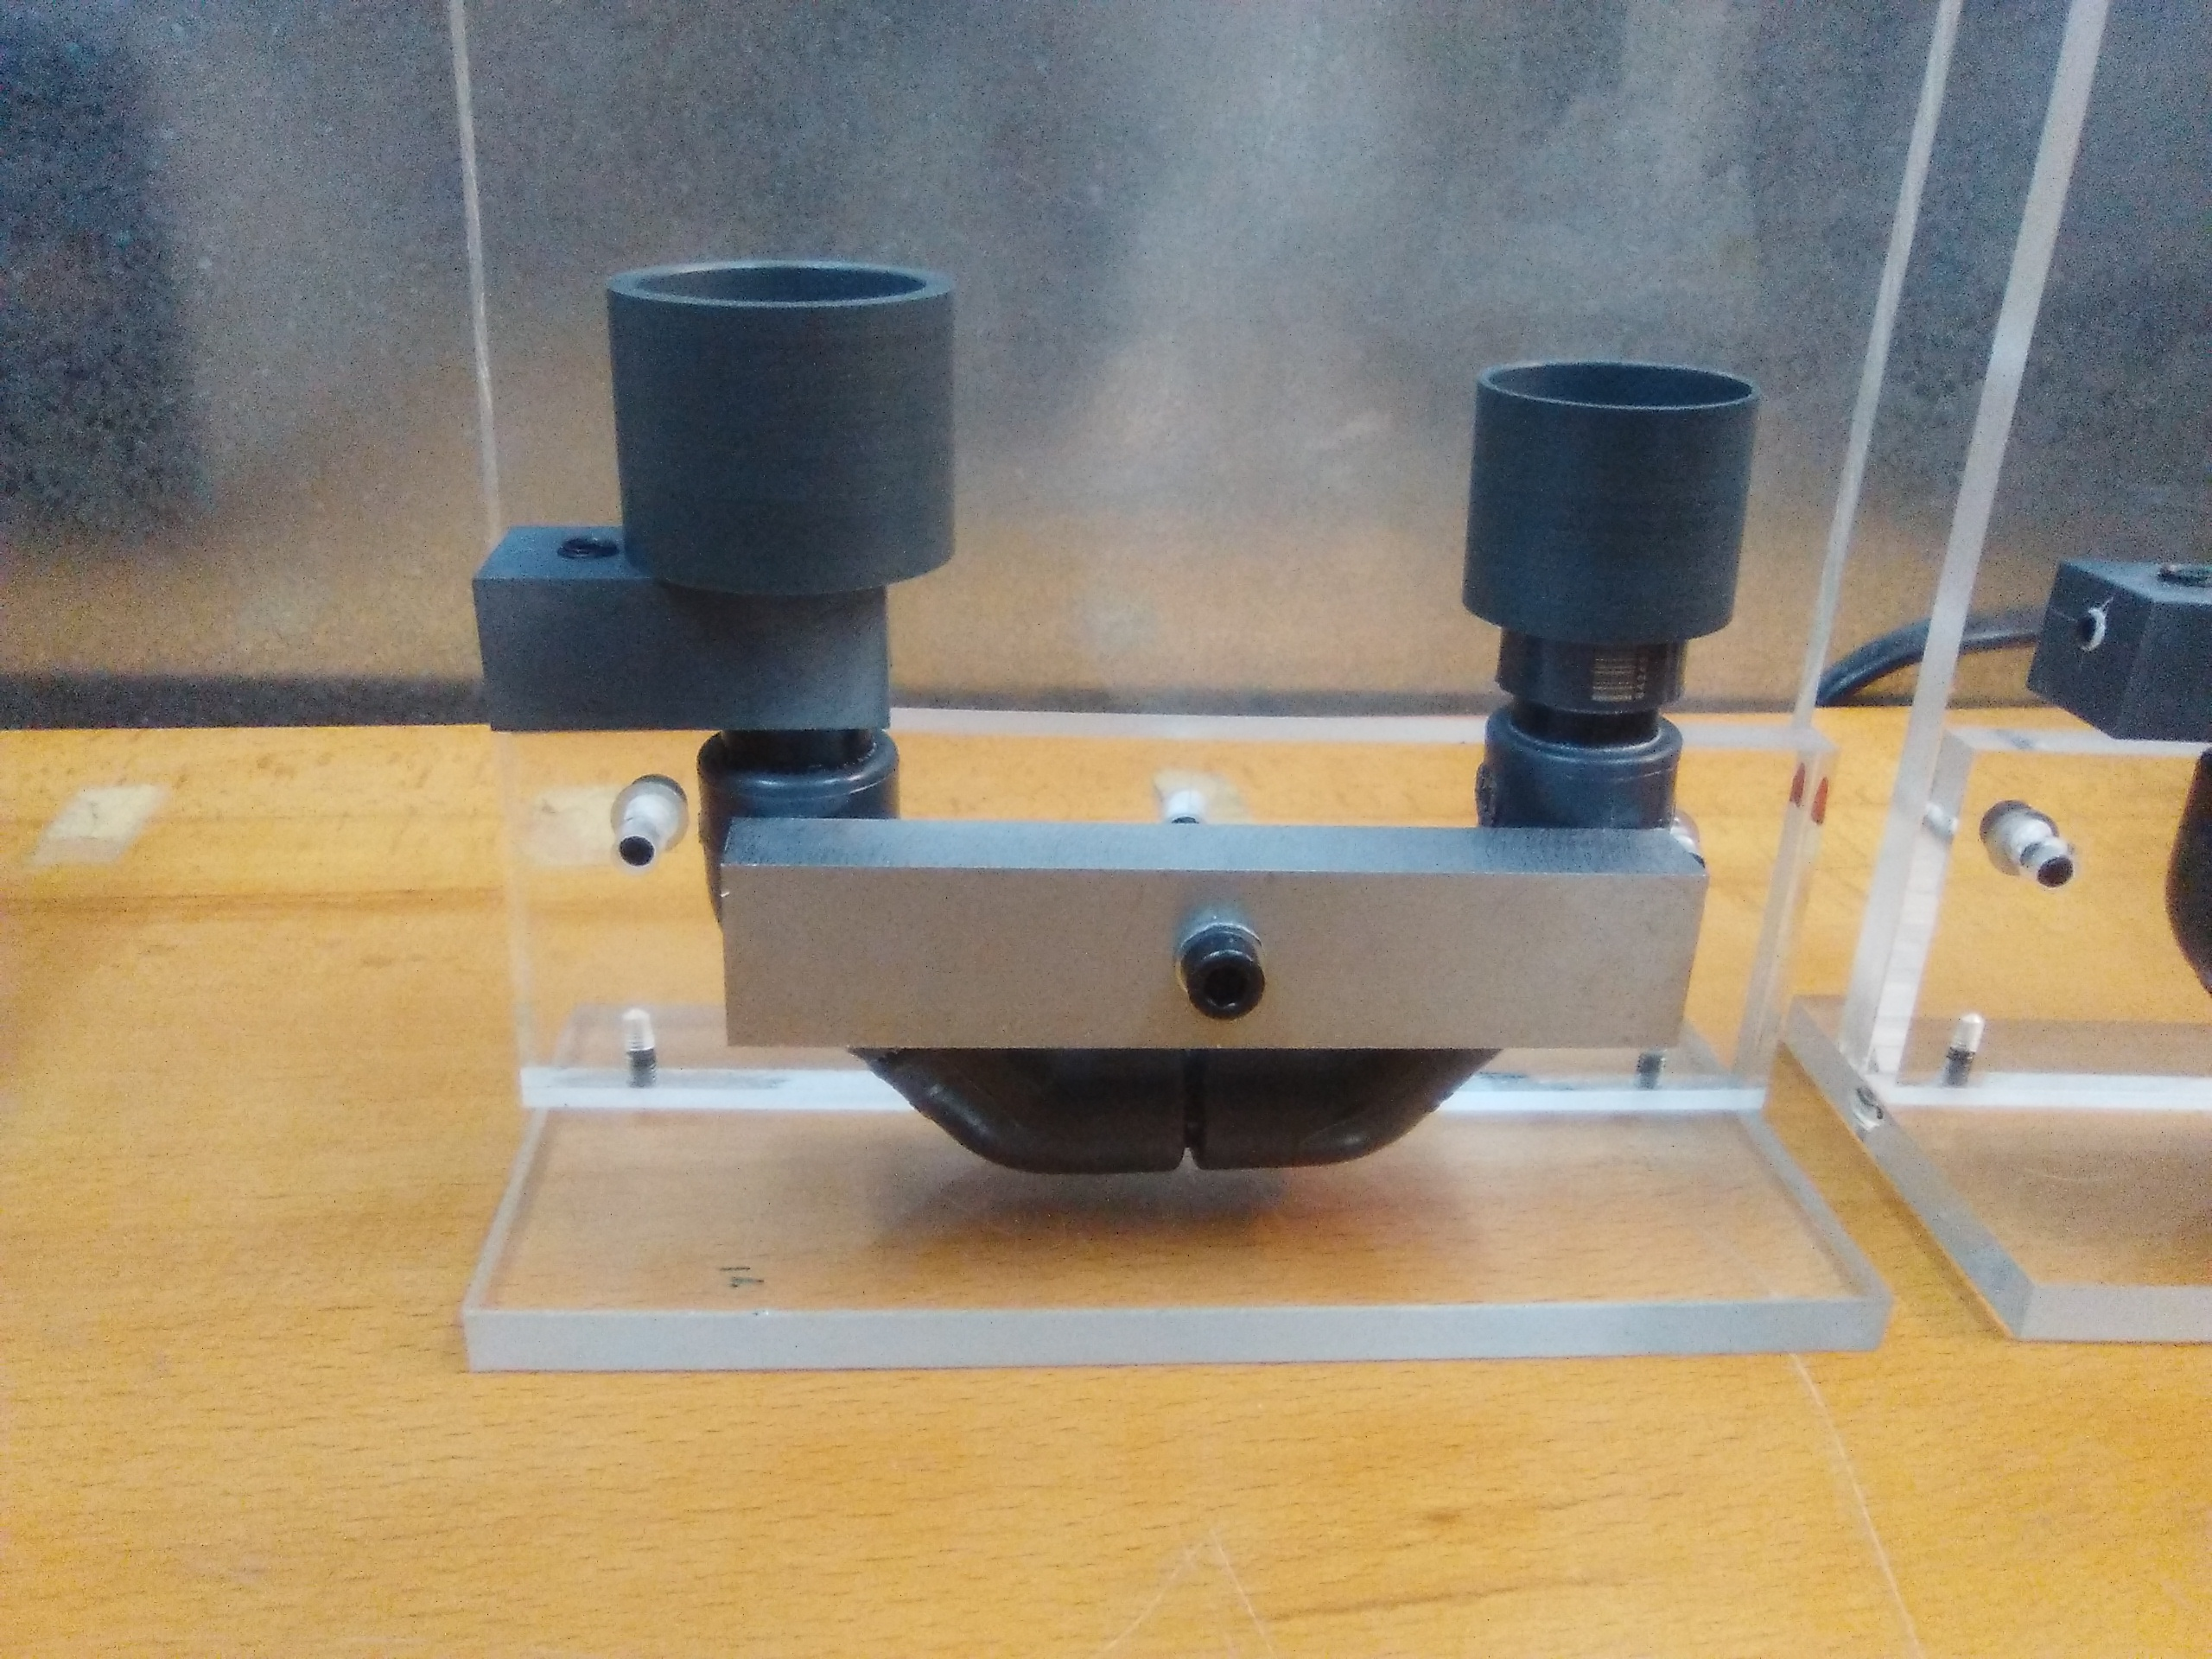
\includegraphics[scale=0.12]{5Prototypes/52PreliminarPrototypes/521TritiumIFIC0/Tritium_IFIC_0.jpg}
\caption{TRITIUM-IFIC-0 Prototype.\label{fig:TritiumIFIC0}}
\end{figure}

Two identical prototypes were built and filled following the same protocol. The first prototype, called ``TRITIUM-IFIC-0 Background'', was filled with pure water ($39~\milli\liter$, uncertainty of $0.05\%$) and was used to measure the background of the detectors whereas the second prototype, called ``TRITIUM-IFIC-0 Signal'', was filled with a radioactive liquid source of tritium, the preparation of which is reported in the appendix \ref{App:TritiumSourcePreparation}. The specific activity of the liquid source employed was $99.696~\kilo\becquerel/\liter$ (uncertainty of $2.24\%$) and the volume used to fill this prototype was the same, $39~\milli\liter$ (uncertainty of $0.05\%$). This second prototype was used to measure the total signal (tritium + background) from the detector. The measured tritium activity was determined by substracting the background from the signal. 

The statistically significant number of time coincident events was found too weak to be measured by time coincidences. The loss of photons was caused by several reasons, such as an excessive curvature of the fiber bundle due to the U-shape of the PVC vessel, causing most of the photons to escape from the fibers and the poor quality of the tritiated water-fiber interface (the cleaning process described in section \ref{subsec:SurfaceConditioningProcess} was motivated by this result). 

A test was carried out to find an explanation to the absence of coincident events in the data. A transparent glass vessel was built similar to the TRITIUM-IFIC-0 prototype vessel, shown in Figure \ref{subfig:PMMAVesselToTestLostPhotons}, to study the effect of the fiber bundle curvature. The LED described in section \ref{subsubsec:CharacterizationFibers} was used to verify the reduction in photocollection efficiency of the fiber bundle due to this curvature. As can be seen in Figure \ref{subfig:TestLostPhotons}, a large amount of photons introduced from one side of the bundle does not reach the other side due to the fiber curvature. This problem indicated the necessity to keep a straight fiber arrangement in the design of the next prototypes. Another important point that can explain the absence of coincident events is the flow of water through the fibers. The fiber bundle of this prototype is very compact and water may not be able to circulate properly around the fibers. This fact will be solved in the next prototype by using a matrix to keep the fibers at a necessary distance.

\begin{figure}
\centering
    \begin{subfigure}[b]{0.45\textwidth}
    \centering
    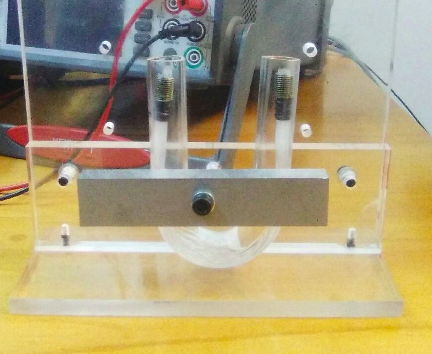
\includegraphics[width=\textwidth]{5Prototypes/52PreliminarPrototypes/521TritiumIFIC0/PMMA_vessel_ZOOM.png}  
    \caption{\label{subfig:PMMAVesselToTestLostPhotons}}
    \end{subfigure}
    \hfill
    \begin{subfigure}[b]{0.45\textwidth}
    \centering
    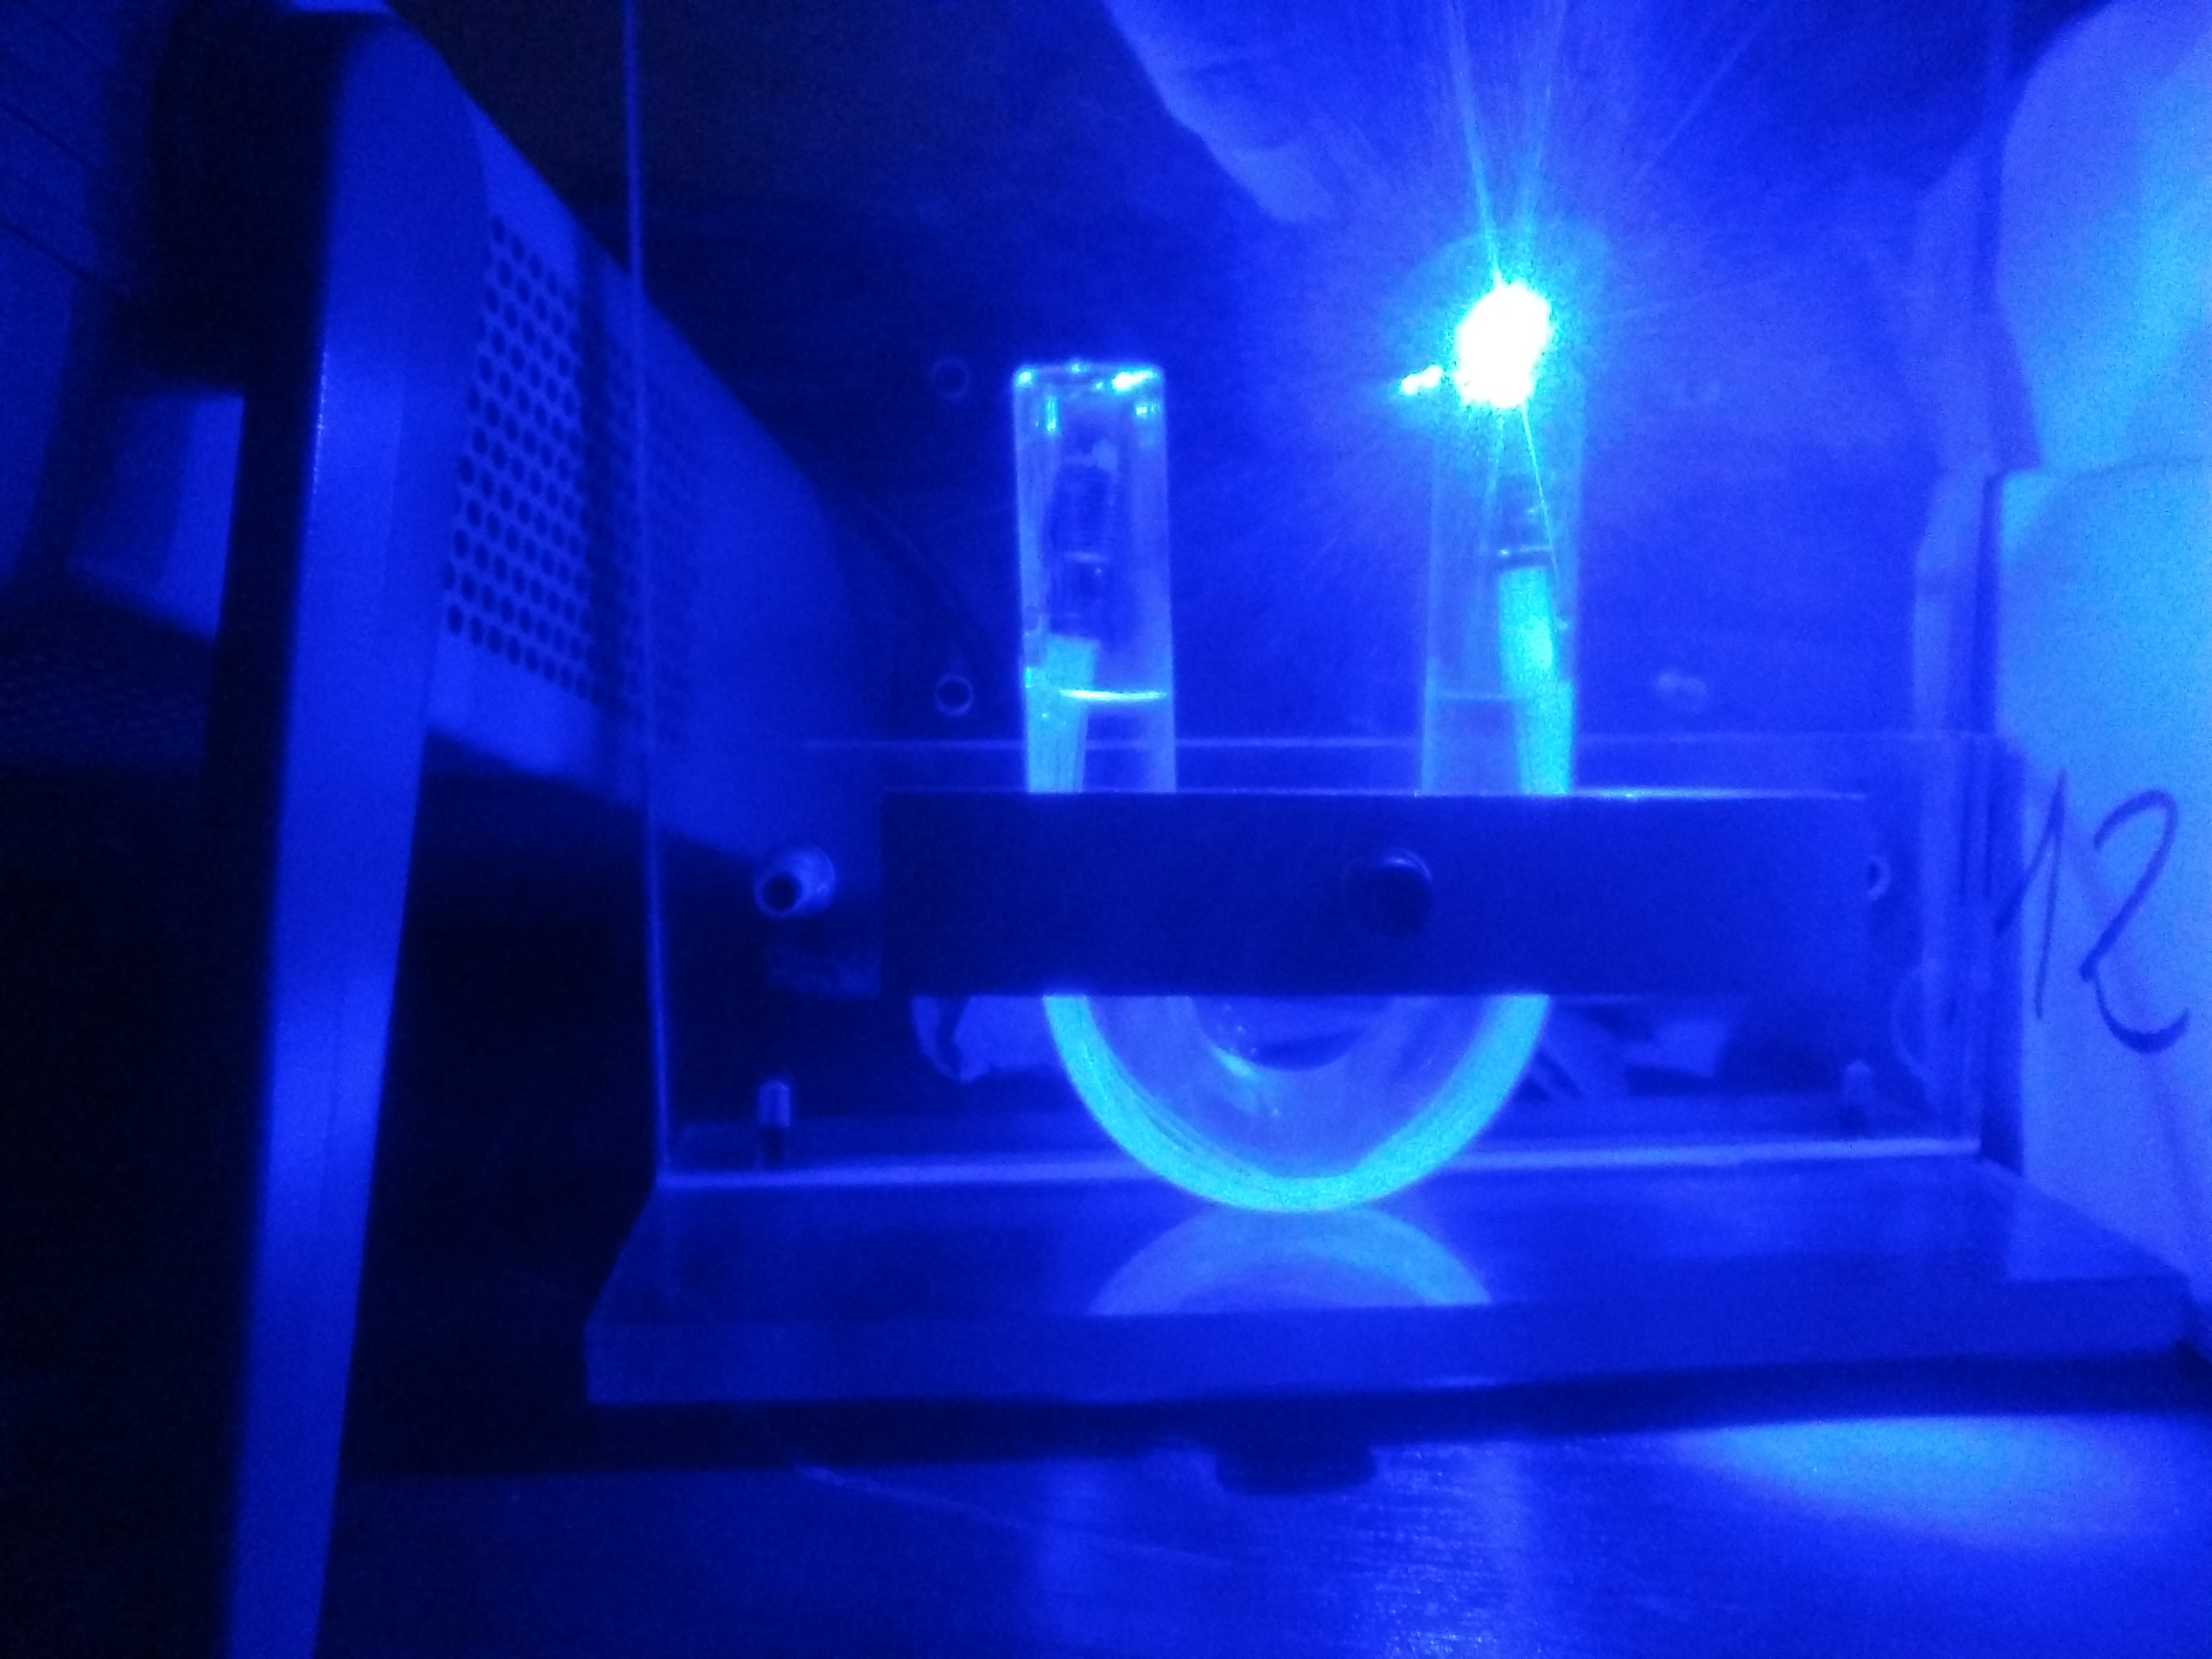
\includegraphics[width=\textwidth]{5Prototypes/52PreliminarPrototypes/521TritiumIFIC0/Lost_Photons.jpg}  
    \caption{\label{subfig:TestLostPhotons}}
    \end{subfigure}
 \caption{a) Fiber bundle in PMMA vessel b) illumination test of the bundle to visualize the light loss due to the fiber curvature.}
 \label{fig:TestLostPhotons}
\end{figure}

To overcome this problem and to obtain some data with this prototype, a single PMT measurement was taken using the electronic chain configuration shown in figure \ref{subfig:ElectronicConfiguraiton1PMT}. The energy spectra measured for both the signal and background prototypes, are shown in Figure \ref{subfig:SignalBackgroundEnergySpectraTritiumIFIC0}. The difference between signal and background, Figure \ref{subfig:TritiumEnergySpectraTritiumIFIC0}, corresponds to the energy spectrum of tritium. The counting rate obtained for the three spectra is given in Table \ref{tab:CountsPerSecondTRITIUMIFIC0}, where the tritium counts are obtained by subtracting the background from the signal.


\begin{figure}
\centering
    \begin{subfigure}[b]{1\textwidth}
    \centering
    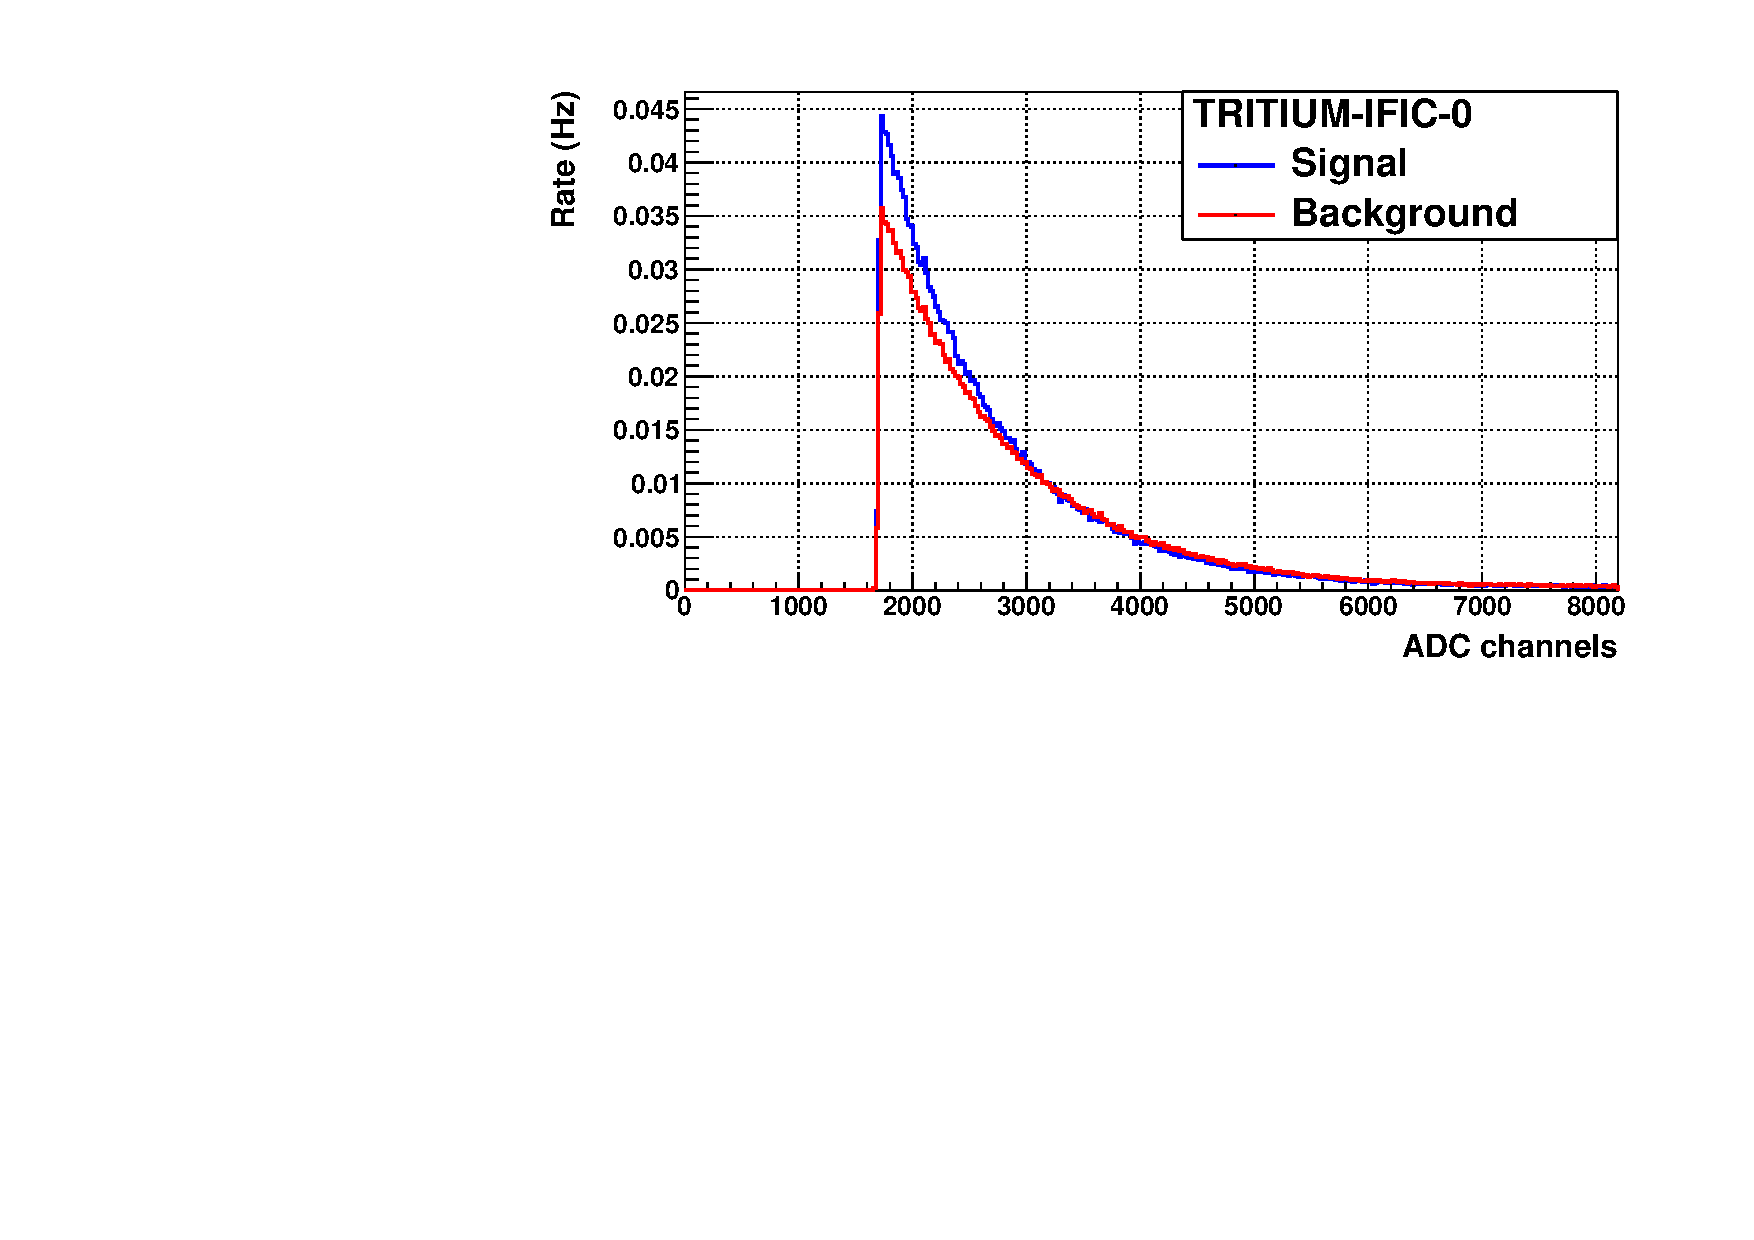
\includegraphics[width=\textwidth]{5Prototypes/52PreliminarPrototypes/521TritiumIFIC0/TritiumIFIC0Signals.pdf}  
    \caption{.\label{subfig:SignalBackgroundEnergySpectraTritiumIFIC0}}
    \end{subfigure}
    \hfill
    \begin{subfigure}[b]{1\textwidth}
    \centering
    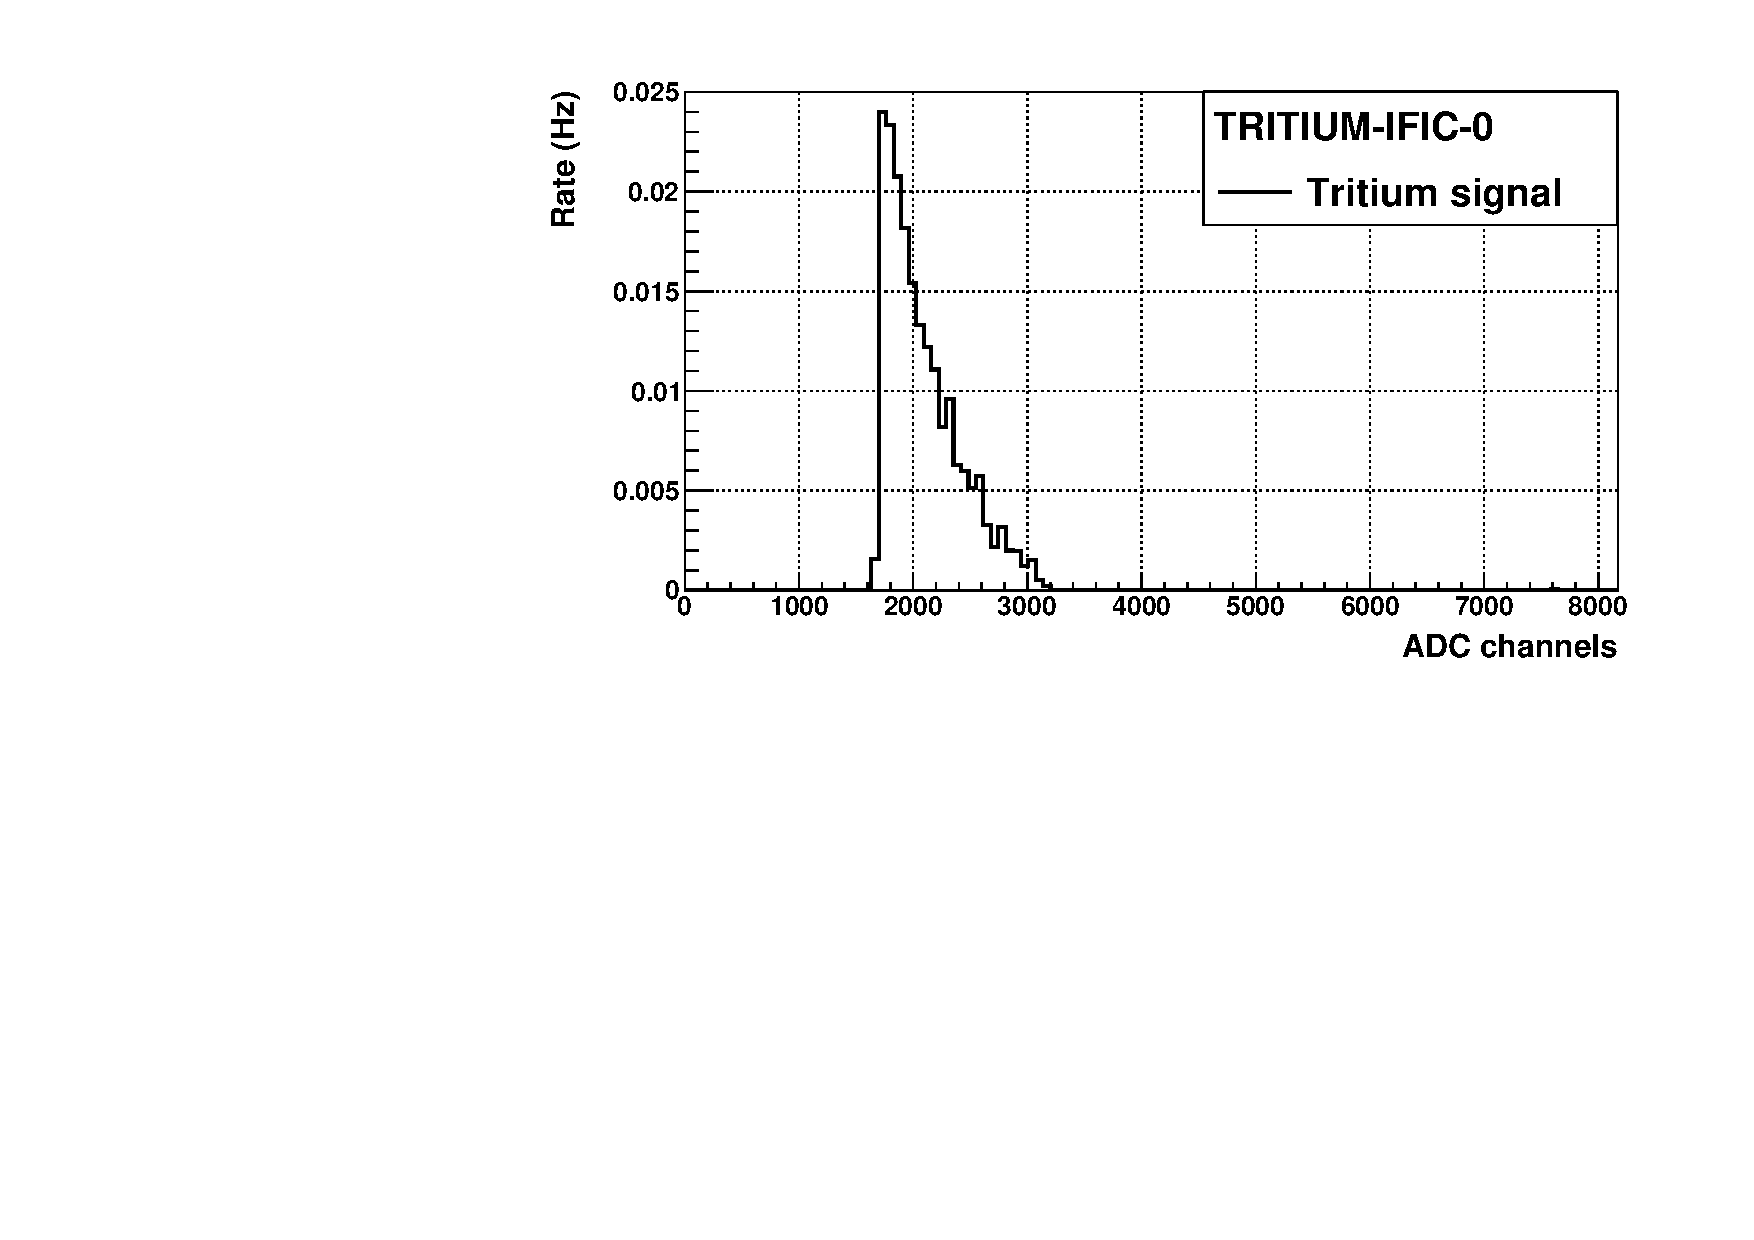
\includegraphics[width=\textwidth]{5Prototypes/52PreliminarPrototypes/521TritiumIFIC0/TritiumIFIC0ClearRebin.pdf}  
    \caption{\label{subfig:TritiumEnergySpectraTritiumIFIC0}}
    \end{subfigure}
 \caption{Energy spectra measured with TRITIUM-IFIC-0 prototype. a) Signal and background energy spectra. b) Tritium energy spectrum.}
 \label{fig:EnergySpectraTRITIUMIFIC0}
\end{figure}

\begin{table}[htbp]
\centering{}%
\begin{tabular}{cc}
\toprule 
Spectrum & Counts/second \tabularnewline
\midrule
\midrule 
Signal prototype & $2.27 \pm 0.06$ \tabularnewline
Background prototype & $2.06 \pm 0.06$ \tabularnewline  
Tritium counts & $0.21 \pm 0.085$ \tabularnewline
\bottomrule
\end{tabular}
\caption{Contes per segon obtinguts per al prototip TRITIUM-IFIC-0.}
\label{tab:CountsPerSecondTRITIUMIFIC0}
\end{table}

The tritium detection efficiency obtained for this prototype is $(2.11 \pm 0.85)\cdot{} 10^{-3}~\frac{cps}{\kilo\becquerel/\liter}$, was calculated as the ratio of the tritium counting rate to the specific activity of the tritium liquid source. 

As we reported in section \ref{sec:StateOfTheArt}, the efficiency of scintillating detectors scales with the active area of the scintillator used. Therefore, to compare the efficiency with oher detectors and with other prototypes developed in TRITIUM experiment, the specific efficiency of this prototype is calculated by normalizing to the scintillator area, which is 
$$S = (9.59 \pm 3.88)\cdot{} 10^{-6}~\frac{cps}{\kilo\becquerel/\liter \cdot{} \cm^{2}}$$
As can be seen in Table \ref{tab:PlasticScinTritium}, the specific efficiency is somewhat larger than that obtained by Muramatsu \cite{Muramatsu}, $3.13 \cdot{} 10^{-6}~\frac{cps}{\kilo\becquerel/\liter \cdot{} \cm^{2}}$, and similar than that obtained by Moghissi \cite{Moghissi}, $ <10.6 \cdot{} 10^{-6}~\frac{cps}{\kilo\becquerel/\liter \cdot{} \cm^{2}}$, both detectors consisting of solid scintillators. These efficiencies are too low efficiencies to achieve the objective of being able to measure $100~\becquerel/\liter$. 





%In addition, some improvements was applied to next prototype, Tritium-IFIC-1. On the one hand, the special cleaning protocol, previously explained in section \ref{subsubsec:CleaningProcess}, was applied on the fibers. It was used to improve the interfaces between fiber and tritiated water, creating a better wetting property of the fiber, which will result in more tritium events detected and a greater photon collection efficiency.

%On the other hand, as we have seen in our previous characterization study of the fibers, shown in section \ref{subsubsec:CharacterizationFibers}, the photon collection efficiency of the fibers used is poor, so a large number of photons will be lost in each tritium event.

%It is an innerent characteristic of the fiber which we cannot change but, to reduce its effect, we will use a Teflon vessel for our next prototypes.

%Teflon is an interesting material for its optical properties, specifically its reflection factor, which is very close to $100\%$ at the working wavelength. It means that practically all the photons that reach the walls of the vessel will be reflected back to the fiber.

%On the other hand, the fibers were inspected under the electronic microscope of the SCSIE \cite{ElectronicMicroscopeSCSIE}, with which we can see details of the order of tens of nanometers.

%The result is shown in Figure \ref{}, where you can see many irregularities of the order of $X~\nm$. These irregularities will cause photons to escape from the fiber. It is a characteristic of the fibers that we cannot change but, to reduce its effect, we will use a Teflon vessel for our next prototypes.

%FOTOOOO

%Teflon is an interesting material for its optical properties, specifically its reflection factor. Its reflection factor is very close to $100\%$ at the working wavelength, which means that practically all the photons that reach walls of the vessel will be reflected back to the fiber.